\documentclass[12pt]{report}
\usepackage[margin=1in]{geometry}
\usepackage[english]{babel}
\usepackage{graphicx}
\usepackage{grffile}

\usepackage{hyperref}
\hypersetup{
    colorlinks=true,
    linkcolor=blue,
    filecolor=magenta,
    urlcolor=blue,
}

\usepackage{listings}
\usepackage{xcolor}

\definecolor{codegreen}{rgb}{0,0.6,0}
\definecolor{codegray}{rgb}{0.5,0.5,0.5}
\definecolor{codepurple}{rgb}{0.58,0,0.82}
\definecolor{backcolour}{rgb}{0.95,0.95,0.92}

\lstdefinestyle{mystyle}{
    backgroundcolor=\color{backcolour},
    commentstyle=\color{codegreen},
    keywordstyle=\color{magenta},
    numberstyle=\tiny\color{codegray},
    stringstyle=\color{codepurple},
    basicstyle=\ttfamily\footnotesize,
    breakatwhitespace=false,
    breaklines=true,
    captionpos=b,
    keepspaces=true,
    numbers=left,
    numbersep=5pt,
    showspaces=false,
    showstringspaces=false,
    showtabs=false,
    tabsize=2
}

\lstset{style=mystyle}

\begin{document}
\title{MSB Final Project: The Genetics of Music}
\author{Kabir Gupta}
\date{\today}
\maketitle

\begin{NoHyper}
\tableofcontents
\end{NoHyper}

\chapter*{Introduction}
\addcontentsline{toc}{part}{Introduction}
One of Tinbergen's four causes of behavior is development, or ontogeny: the question of how a behavior came to an organism in the first place.\footnote{Special thanks to Lincoln Auster and Thomas Morford for code review, bug fixes and formatting advice.} While this subject can delve deep into Mendellian inheritance and meiosis, or different forms of learning and different classifications of innate behaviors, the most basic and central question asked during the study of development is that of nature versus nurture: is the trait genetically inherited or environmentally acquired? Of course, traits are often not one or the other but will rather fall on a spectrum between the two; the purpose of this project is to study one such trait in hopes of determining whether it is influenced more by genes or environment. This trait is musical taste: what kinds of music do people like to listen to?

It is surprisingly common, in the researcher's own (anecdotal) experience, to find two friends who have vastly different music tastes, and the same applies to family members. This leads into the question of who makes more of an impact on your music tastes --- friends will often attest to have virtually identical music taste, but the same could apply to family members; it only seems to vary from person to person and family to family. By gathering a large sample of data, however, it could be determined whether there is actually some sort of trend: an association between a person's music tastes and their friends'/family's.

It was expected that both family members and friends would have a significant impact on a person's music choices, although one might not necessarily outweigh the other: that is, there may not be a significant difference between the family's impact and the friends'. This is because people have very strong reasons to like similar music to both a family member and a friend, so that one relationship type should not be significantly closer than the other.

\chapter*{Materials and Methods}
\addcontentsline{toc}{part}{Materials and Methods}
A Google Forms survey was used to gather data for this study, and a Python script was used to analyze it (included in Appendix I). Each respondent was asked to select the musical genres that they enjoy out of 6 options: pop, jazz/blues, rock, country/folk, rap/hip hop, and classical. The respondent was then asked to decide whether they like or dislike each of 12 musical clips, out of which each genre was represented by two clips: Uptown Funk and Dead Girl in the Pool (pop), What a Wonderful World and The Thrill is Gone (jazz and blues), Bohemian Rhapsody and Hurt (rock), Old Town Road and I Walk the Line (country and folk), Rap God and Gangsta's Paradise (rap and hip hop), and finally Eine Kleine Nachtmusik and Duel of the Fates (classical).

For the purposes of this study, it was useful to be able to identify whether there were some genres that the respondent did not necessarily dislike, even if it was not something they thought they actively listen to. So, while the first part of the survey asked for what they thought they like, the second part of the survey was in an attempt to see what they might actually like. However, it's possible that somebody who generally likes a certain genre did not like the specific two clips that they had been asked about from that genre. So, the question about categories needed to be weighted more heavily than the questions about specific songs. Further, an overall system was needed for condensing the 2-part data that would be gathered --- genre and music preference, both on nominal scales --- into one number that could be used in statistical testing. Hence, the following scoring system was created, as seen in Figure 1.

\begin{figure}[h!]
  \centerline{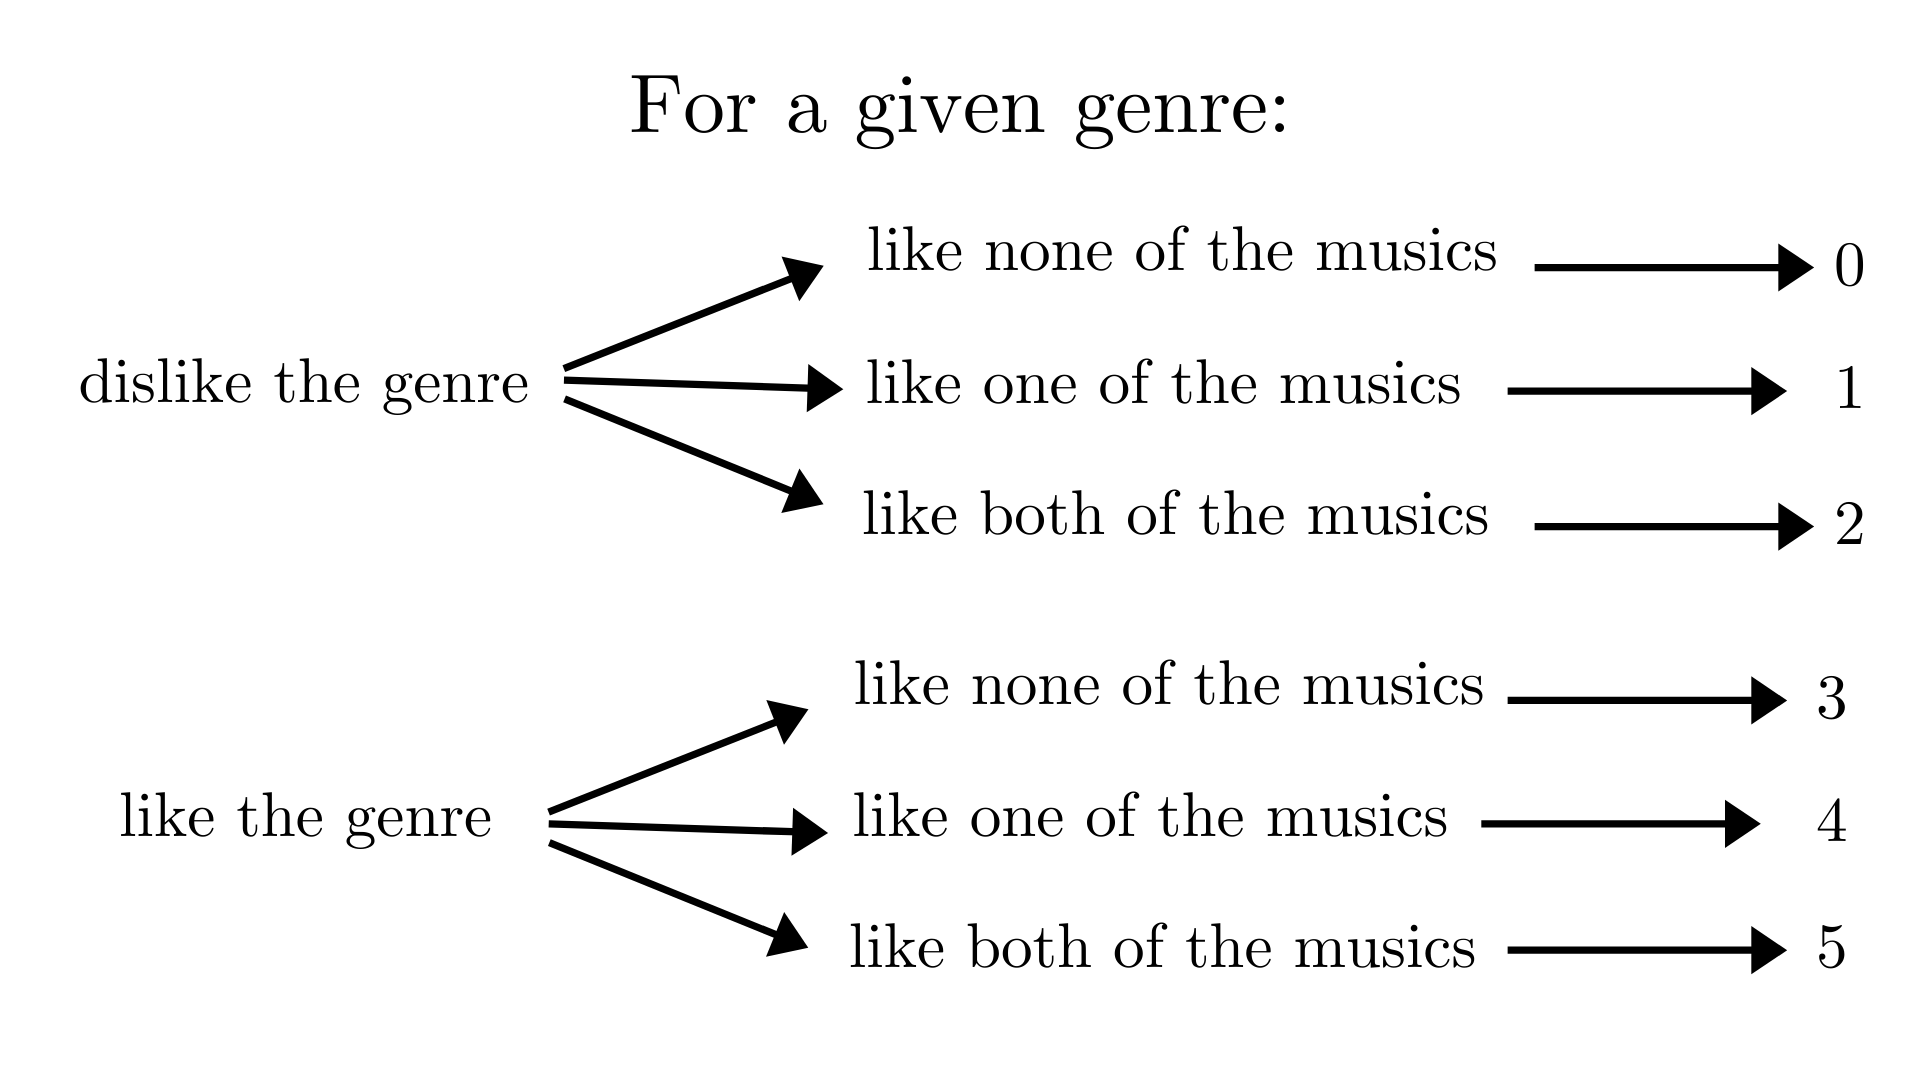
\includegraphics[width=0.5\linewidth]{matrix.png}}
  \caption{\small The procedure used to generate ordinal-scale scores for each respondent, for each genre.}
\end{figure}

This means that if a respondent says they enjoy a particular genre but doesn't like any of the musics, they can still walk away with a score of 3, whereas if they liked both musics but said they disliked the genre in general, they would only get a 2. These rankings are on an ordinal scale, from 0 to 5 (where there are no defined intervals between ranks).

Each respondent was requested to provide the names of two friends and two family members. The family members were sent a slightly different survey, which was identical to the one for students except that it did not ask them for the names of their friends or family members. At the end of data collection, each respondent was matched up to their two family members and two friends to perform statistical analysis. If not all of the family members and friends listed had responded to the survey, only the ones whose responses were present were tested against the student.

\chapter*{Data}
\addcontentsline{toc}{part}{Data}
There were two main variables being compared in this study: relationship type (family member or friend), on a nominal (binary) scale; and genre rankings that demonstrate the degree to which someone enjoys a particular genre, on an ordinal scale.

\begin{figure}[h!]
  \centerline{\includegraphics[width=0.5\textwidth]{"Genre 1"}}
  \caption{\small Scatter plot displaying the data gathered for Genre \#1, pop music. Here, the absolute difference between the student's ratings and their family member's (median if both family members responded) (x) is plotted against the absolute difference between the student's ratings and their friend's (again, median if both friends responded).}
\end{figure}

\begin{figure}[h!]
  \centerline{\includegraphics[width=0.5\textwidth]{{"Genre 2"}.png}}
  \caption{\small Similar to above, scatter plot for Genre \#2, jazz and blues.}
\end{figure}

\begin{figure}[h!]
  \centerline{\includegraphics[width=0.5\textwidth]{{"Genre 3"}.png}}
  \caption{\small Scatter plot for Genre \#3, rock music.}
\end{figure}

\begin{figure}[h!]
  \centerline{\includegraphics[width=0.5\textwidth]{{"Genre 4"}.png}}
  \caption{\small Scatter plot for Genre \#4, country and folk.}
\end{figure}

\begin{figure}[h!]
  \centerline{\includegraphics[width=0.5\textwidth]{{"Genre 5"}.png}}
  \caption{\small Scatter plot for Genre \#5, rap and hip hop.}
\end{figure}

\begin{figure}[h!]
  \centerline{\includegraphics[width=0.5\textwidth]{{"Genre 6"}.png}}   
  \caption{\small Scatter plot for Genre \#6, classical music.}
\end{figure}

The scatter plots above (Figures 2-7) display the results of data collection, spread across genres. The raw data gathered during this study is included in Appendix II.

A Wilcoxon test was used for the primary statistical analysis. Out of 49 tests conducted for a difference between the students' rankings and their family members', 9 were statistically significant at a 90\% confidence level (a=0.10), and 5 were significant at a 95\% confidence level (a=0.05). For the friends, 14 tests came out significant at the 90\% confidence level, and 7 at the 95\% confidence level, out of a total of 79 tests. Overall, 18.4\% of tests conducted for family members came back significant, compared to 17.7\% of tests for friends.

The follow-up chi-square test for association had an insignificant result, meaning that the null hypothesis must be accepted: there is no association between relationship type and similarity of rankings. The test statistic $\chi^2$ was calculated to be 3.389771795679717 with 9 degrees of freedom; p=0.9468207928306335.

A Spearman-rank correlation coefficient (SRCC) was also calculated for each relationship type for each genre. For family members, the correlation coefficients were r = 0.48, 0.05, -0.10, 0.13, 0.21, and -0.15 respectively. For friends, they were r = 0.21, 0.21, 0.07, 0.04, -0.03, and 0.06 respectively. Three of the coefficients overall (two on the family side and one on the friends side) were negative; all the rest were positive. Almost all of the correlation coefficients were quite weak (below 0.1); however, the correlation coefficient for Genre 1 (Pop) for family members could be classified as of moderate strength. Apart from the aforementioned coefficient, which had a p-value p=0.00679 (highly statistically significant), all the other coefficients were insignificant.

Finally, a t-test for two correlated samples was conducted between the family members' and friends' correlation coefficients to test for a significant difference in the correlation coefficients. The test statistic reported was t = 0.14. The critical value for the t-distribution at a 95\% confidence level with 5 degrees of freedom is 2.57, and the test statistic found does not exceed this. The p-value was only p = 0.90, so the result was insignificant. Thus, we fail to reject the null hypothesis that family members and friends both influence people's musical choices to approximately the same extent.

\chapter*{Statistical Analysis}
\addcontentsline{toc}{part}{Statistical Analysis}
The most preliminary technique used in analyzing the collected data was assigning each individual an ordinal-scale ranking for each genre (in order to have two easily comparable populations). The specifications of how this was done have been provided in the Methods section. Once each student, family member and friend was assigned a set of 6 ranks (as there were 6 genres involved), a comparison of medians was conducted between the data sets. Because the data was on an ordinal scale, the statistical test had to be nonparametric. Further, the data was paired because each student was related to their corresponding family member or friend in some way. Consequently, a Wilcoxon test was used to test for a significant difference between each student's rankings and their family members', and between each student's rankings and their friends'. The results of these tests are summarized in the previous section.

The p-values generated by the Wilcoxon tests were sorted into an aggregated frequency table (class borders 0-0.1, 0.1-0.2, 0.2-0.3, and so on up to 1.0). This was done to each set of tests (family and friends), allowing for the construction of the contingency tables below (Tables 1 and 2). A chi-square test for association was conducted to find if there was an association between to what extent two people differ in music choice, and how the two people are related (family or friend).

\begin{table}[h!]
\begin{center}

\begin{tabular}{ c|c|c|c|c|c|c|c|c|c|c }
  & \textbf{0.1} & \textbf{0.2} & \textbf{0.3} & \textbf{0.4} & \textbf{0.5} & \textbf{0.6} & \textbf{0.7} & \textbf{0.8} & \textbf{0.9} & \textbf{1.0} \\ 
  \hline \hline
  \textbf{Family} & 9 & 11 & 3 & 5 & 6 & 1 & 3 & 6 & 2 & 3\\
  \hline
  \textbf{Friend} & 14 & 16 & 8 & 4 & 10 & 5 & 4 & 9 & 5 & 4 \\
\end{tabular}

\caption{Contingency table of observed values for $\chi^2$}

\vspace{20pt}

\begin{tabular}{ c|c|c|c|c|c|c|c|c|c|c }
  & \textbf{0.1} & \textbf{0.2} & \textbf{0.3} & \textbf{0.4} & \textbf{0.5} & \textbf{0.6} & \textbf{0.7} & \textbf{0.8} & \textbf{0.9} & \textbf{1.0} \\
  \hline \hline
  \textbf{Family} & 8.80 & 10.34 & 4.21 & 3.45 & 6.13 & 2.30 & 2.68 & 5.74 & 2.68 & 2.6 \\
  \hline
  \textbf{Friend} & 14.20 & 16.66 & 6.79 & 5.55 & 9.88 & 3.70 & 4.32 & 9.26 & 4.32 & 4.32 \\
\end{tabular}

\caption{Contingency table of expected values for $\chi^2$}

\end{center}
\end{table}

Although the chi-square test returned an insignificant result, it was still worth calcualting a Spearman-rank correlation coefficient to get a sense of how strong the correlation between each pair of two people was for each genre. This gave a set of twelve SRCCs, one for each genre and for each relationship type (friend/family). The SRCC comparison tables were of the format as in Table 3 (only a part of the first one is included here, as they were all similarly structured.)

\begin{table}[h!]
\begin{center}
\begin{tabular}{ c|c }
 x: student's ranking & y: family member's ranking \\
 \hline
 0 & 4 \\
 \hline
 1 & 0 \\
 \hline
 1 & 0 \\
 \hline
 ... & ... \\
 \hline
\end{tabular}
\caption{SRCC table of values for students vs family members for Genre 1, Pop (truncated after row 3).}
\end{center}
\end{table}

The twelve correlation coefficients that were found (six for each relationship type) have been reported in the previous section. One last statistical test was conducted, the t-test for two correlated (paired) samples. A significant result here would have meant that one relationship type (be that family member or friend) has significantly higher correlations between two people than the other. The two samples consisted of the set of all SRCCs for family members, and the set of all SRCCs for friends (thus n=6). So, each sample was matched because every SRCC for the family members applied to the same genre as the corresponding SRCC for the friends. Further, a parametric test could be used because correlation coefficients lie on a ratio scale (with an absolute zero) and there was no reason to suspect major skew in the data. The results of the two-sample t-test were reported in the previous section as well.

\chapter*{Discussion}
\addcontentsline{toc}{part}{Discussion}
Conducting the Wilcoxon tests for each student revealed that there were some cases where there was a significant difference between family members, and likewise for friends. However, when all of those cases were tallied up in a chi-square test, there did not appear to be a significant association between relationship type and music choices. While calculating the SRCCs supported this conclusion for the most part, one of the coefficients did suggest that family members may exert a special influence on students' choices when it comes to pop music based on the correlation coefficient alone. However, when a t-test was run between the SRCCs to check for a significant difference, the result was clear: neither relationship has greater power over a person's musical choices than the other.

The data gathered thus supports the original hypothesis that an environmental influence would not outweigh a genetical influence on a person's music choices, and vice versa. However, there are two ways these results could have been made more reliable:

\begin{itemize}
  \item A larger sample size always helps increase the power of statistical analysis, and can thus catch smaller differences in a population that a small sample size cannot. The sample size for this study was 76 students and 65 family members; while that's not a tiny sample size, this study would definitely have been more powerful if (a) more people participated, but even more so (b) for every student who participated, both family members and both friends were able to fill out the respective surveys.
  \item The twelve songs selected to ``represent'' each genre may not have been very representative of each genre. For instance, ``Hurt'' is a heavy metal song that even an avid rock listener might not find as appealing as a pure rock song. ``Eine Kleine Nachtmusik,'' while popular, is overused to the point of many classical enthusiasts not enjoying it as much as some Brahms or Shostakovich; and ``Duel of the Fates'' is a vocalized theme from the \textit{Star Wars} soundtrack, so that it can technically be categorized as classical but when compared to Bach or Beethoven seems vastly different. These oversights were due to the researcher's own relative lack of musical knowledge (which has slightly improved over the course of this study).
\end{itemize}

A redo of this study could have the potential to be more successful if more time was spent to take as large a sample size as possible --- for instance, if everybody in one school filled it out, it might only provide 500 people, but at least each person's friend would have (hopefully) filled it out too until it cycled back so that every person can be tested against four other people --- and to use music clips that were much more representative of the genre (and likely to be liked by somebody who listens to the genre often).

Another possible flaw in this research was that it assumes that family members are the ``genetic'' factor, and friends are the ``environmental''. While it's true that there's usually no genetic relationship between two friends, the problem is that one's family is not only who they share the greatest amount of their DNA with, but also who they have usually grown up around and been brought up with. This means that a family member might encapsulate both the genetic and the environmental factor. Thus, this study cannot really conclude whether music has a large genetic part, because it is quite possible that the overlaps found between students and their family members were due to a shared environment --- in some cases, people may even share much more of their environment with family members than with friends. To rectify this, a completely different study might need to be carried out, maybe one connecting genetically related people who have not been in the same environment (cousins? siblings who were separated at birth? long-lost parents or children? clones?) might be more powerful in revealing whether there is more of a genetic and an environmental factor at play.

\chapter*{References}
\addcontentsline{toc}{part}{References}
A Google Forms survey was used in this study, and the data was linked into a Google Sheet spreadsheet. The following twelve songs were used during the study; the relevant portions were clipped out (10 seconds) for survey-takers to listen to.

\begin{enumerate}
  \item ``Uptown Funk'', Mark Ronson, 00:58 to 1:08. \url{https://youtu.be/OPf0YbXqDm0}
  \item ``Dead Girl in the Pool'', girl in red, 00:34 to 00:44. \url{https://youtu.be/Pzq4TEU-wHo}
  \item ``What a Wonderful World'', Louis Armstrong, 00:17 to 00:27. \url{https://youtu.be/VqhCQZaH4Vs}
  \item ``The Thrill is Gone'', B.B. King, 00:34 to 00:44. \url{https://youtu.be/oica5jG7FpU}
  \item ``Bohemian Rhapsody'', Queen, 00:02 to 00:12. \url{https://youtu.be/fJ9rUzIMcZQ}
  \item ``Hurt'', Nine Inch Nails, 4:01 to 4:11. \url{https://youtu.be/OvoTktdpIiI}
  \item ``Old Town Road'', Lil Nas X, 00:39 to 00:49. \url{https://youtu.be/r7qovpFAGrQ}
  \item ``I Walk the Line'', Johnny Cash, 00:25 to 00:35. \url{https://youtu.be/J5126CibNsk}
  \item ``Rap God'', Eminem, 00:25 to 00:35. \url{https://youtu.be/XbGs_qK2PQA}
  \item ``Gangsta's Paradise'', Coolio, 00:57 to 1:07. \url{https://youtu.be/fPO76Jlnz6c}
  \item ``Eine Kleine Nachtmusik'', Wolfgang Amadeus Mozart, 00:05 to 00:15. \url{https://youtu.be/oy2zDJPIgwc}
  \item ``Duel of the Fates'', John Williams, 1:03 to 11:13. \url{https://youtu.be/C2XUJ5PWg-8}
\end{enumerate}

For the Python script, the SciPy Statistics library (\texttt{scipy==1.6.3}) was used to perform statistical analyses. The Pandas library (\texttt{pandas==1.2.4}) was used to import data from a CSV (exported from Google Sheets) into the Python script. Finally, the Matplotlib library (\texttt{matplotlib==3.4.2}) was used to draw scatter plots from the data collected.

\chapter*{Appendix I}
\addcontentsline{toc}{part}{Appendices}
\addcontentsline{toc}{chapter}{Appendix I}
The following scripts were used to analyze the data gathered.

Main program:

\lstinputlisting[language=Python]{main.py}

Wrapper script (using POSIX sh):

\lstinputlisting[language=sh]{wrapper.sh}

Class definitions for students and families:

\lstinputlisting[language=Python]{people.py}

\chapter*{Appendix II}
\addcontentsline{toc}{chapter}{Appendix II}
On the following two pages are presented the raw data collected over the course of study. In order to protect the privacy of those participating in the study, respondents' first and last names have been entirely ommitted, and their friends' and family members' names have been replaced with the unique timestamps associated with that person's response. The first table displays raw data for students (including friends), and the second for family members.

\newgeometry{left=0.1cm,right=0.1cm}
\begin{table}
    \centering
    \begin{tabular}{|l|l|l|l|l|l|l|l|l|l|l|l|l|l|l|l|l|l|l|l|l|l|}
    \hline
        Timestamp & Check all of the following which you enjoy listening to: & Music \#1 Opinion & Music \#2 Opinion & Music \#3 Opinion & Music \#4 Opinion & Music \#5 Opinion & Music \#6 Opinion & Music \#7 Opinion & Music \#8 Opinion & Music \#9 Opinion & Music \#10 Opinion & Music \#11 Opinion & Music \#12 Opinion & Last Name of Family Member \#1 & First Name of Family Member \#1 & Last Name of Family Member \#2 & First Name of Family Member \#2 & Last Name of Friend \#1 & First Name of Friend \#1 & Last Name of Friend \#2 & First Name of Friend \#2 \\ \hline
        3/30/2021 18:25:03 & Pop, Rock, Classical & Like & Dislike & Like & Dislike & Like & Dislike & Dislike & Like & Dislike & Dislike & Like & Like & 3/31/2021 20:35:02 & 3/31/2021 20:35:02 & 3/31/2021 20:34:23 & 3/31/2021 20:34:23 & 5/17/2021 12:54:35 & 5/17/2021 12:54:35 & 3/30/2021 19:08:20 & 3/30/2021 19:08:20 \\ \hline
        3/30/2021 19:04:10 & Pop, Rock, Classical & Dislike & Like & Like & Dislike & Like & Like & Like & Dislike & Dislike & Like & Like & Dislike & 5/9/2021 22:40:12 & 5/9/2021 22:40:12 &  &  & 5/9/2021 22:47:55 & 5/9/2021 22:47:55 & 5/9/2021 22:45:20 & 5/9/2021 22:45:20 \\ \hline
        3/30/2021 19:08:20 & Pop, Jazz/Blues, Rap/Hip Hop, Classical & Like & Like & Like & Dislike & Like & Dislike & Like & Dislike & Like & Like & Like & Like & 3/30/2021 19:48:57 & 3/30/2021 19:48:57 & 3/30/2021 19:11:45 & 3/30/2021 19:11:45 & 5/17/2021 12:54:35 & 5/17/2021 12:54:35 & 3/27/2021 13:30:39 & 3/27/2021 13:30:39 \\ \hline
        3/30/2021 19:16:50 & Pop, Rap/Hip Hop, Classical & Like & Like & Like & Dislike & Dislike & Like & Dislike & Dislike & Like & Like & Dislike & Dislike &  &  &  &  & 4/11/2021 18:49:19 & 4/11/2021 18:49:19 &  &  \\ \hline
        3/30/2021 19:38:17 & Pop, Rap/Hip Hop, Classical & Like & Like & Dislike & Dislike & Dislike & Dislike & Like & Dislike & Like & Like & Like & Dislike & 5/10/2021 8:33:11 & 5/10/2021 8:33:11 &  &  &  &  &  &  \\ \hline
        3/30/2021 19:43:52 & Pop, Classical & Dislike & Dislike & Dislike & Dislike & Dislike & Dislike & Dislike & Dislike & Dislike & Dislike & Dislike & Dislike &  &  &  &  & 3/30/2021 19:47:44 & 3/30/2021 19:47:44 & 3/30/2021 20:49:59 & 3/30/2021 20:49:59 \\ \hline
        3/30/2021 19:47:44 & Pop, Country/Folk, Rap/Hip Hop, Classical & Like & Like & Like & Like & Like & Like & Dislike & Dislike & Like & Like & Like & Dislike & 5/13/2021 10:04:34 & 5/13/2021 10:04:34 & 3/30/2021 20:01:45 & 3/30/2021 20:01:45 & 3/30/2021 19:43:52 & 3/30/2021 19:43:52 & 3/30/2021 20:49:59 & 3/30/2021 20:49:59 \\ \hline
        3/30/2021 19:57:52 & Pop, Rap/Hip Hop & Dislike & Dislike & Dislike & Dislike & Like & Dislike & Like & Dislike & Like & Like & Dislike & Dislike & 5/10/2021 7:58:09 & 5/10/2021 7:58:09 & 5/10/2021 8:32:01 & 5/10/2021 8:32:01 & 5/17/2021 12:54:35 & 5/17/2021 12:54:35 & 5/9/2021 22:22:38 & 5/9/2021 22:22:38 \\ \hline
        3/30/2021 20:39:10 & Pop, Rock, Classical & Like & Like & Like & Dislike & Like & Dislike & Dislike & Dislike & Like & Dislike & Like & Dislike & 5/10/2021 6:44:47 & 5/10/2021 6:44:47 & 3/30/2021 20:44:13 & 3/30/2021 20:44:13 &  &  &  &  \\ \hline
        3/30/2021 20:49:59 & Rock & Dislike & Dislike & Like & Dislike & Like & Like & Dislike & Like & Dislike & Dislike & Like & Dislike & 3/30/2021 21:56:23 & 3/30/2021 21:56:23 &  &  & 3/30/2021 19:43:52 & 3/30/2021 19:43:52 & 3/30/2021 19:47:44 & 3/30/2021 19:47:44 \\ \hline
        3/31/2021 1:00:09 & Pop, Jazz/Blues, Rock, Country/Folk, Rap/Hip Hop, Classical & Like & Like & Like & Like & Dislike & Dislike & Like & Like & Like & Like & Like & Like &  &  &  &  & 5/12/2021 22:07:21 & 5/12/2021 22:07:21 & 5/10/2021 0:22:24 & 5/10/2021 0:22:24 \\ \hline
        3/31/2021 6:47:05 & Rock, Classical & Like & Dislike & Like & Dislike & Like & Dislike & Dislike & Dislike & Dislike & Dislike & Like & Like &  &  & 5/10/2021 16:28:12 & 5/10/2021 16:28:12 & 3/30/2021 19:08:20 & 3/30/2021 19:08:20 & 4/20/2021 19:44:09 & 4/20/2021 19:44:09 \\ \hline
        3/31/2021 7:56:24 & Pop, Jazz/Blues, Country/Folk, Classical & Like & Dislike & Like & Dislike & Like & Dislike & Like & Dislike & Dislike & Dislike & Like & Dislike &  &  &  &  &  &  & 3/31/2021 23:14:02 & 3/31/2021 23:14:02 \\ \hline
        3/31/2021 11:29:15 & Pop, Rock, Rap/Hip Hop & Like & Dislike & Like & Dislike & Like & Like & Dislike & Dislike & Dislike & Like & Dislike & Dislike & 3/31/2021 11:36:00 & 3/31/2021 11:36:00 & 3/31/2021 13:59:28 & 3/31/2021 13:59:28 & 3/31/2021 15:45:07 & 3/31/2021 15:45:07 & 3/31/2021 23:14:02 & 3/31/2021 23:14:02 \\ \hline
        4/20/2021 19:44:09 & Pop, Jazz/Blues, Classical & Like & Dislike & Like & Dislike & Like & Dislike & Dislike & Like & Dislike & Dislike & Like & Like &  &  &  &  & 3/31/2021 17:19:58 & 3/31/2021 17:19:58 & 3/31/2021 6:47:05 & 3/31/2021 6:47:05 \\ \hline
        3/31/2021 12:45:53 & Pop & Like & Dislike & Like & Like & Like & Dislike & Like & Dislike & Dislike & Dislike & Like & Dislike & 3/30/2021 19:09:14 & 3/30/2021 19:09:14 & 3/30/2021 19:15:42 & 3/30/2021 19:15:42 & 3/30/2021 20:27:00 & 3/30/2021 20:27:00 & 3/31/2021 11:14:22 & 3/31/2021 11:14:22 \\ \hline
        3/31/2021 12:54:02 & Jazz/Blues, Classical & Like & Dislike & Like & Like & Dislike & Dislike & Dislike & Dislike & Dislike & Dislike & Like & Like & 3/31/2021 22:32:00 & 3/31/2021 22:32:00 & 3/31/2021 13:01:20 & 3/31/2021 13:01:20 &  &  &  &  \\ \hline
        3/31/2021 14:19:59 & Pop, Rock, Classical & Like & Like & Like & Dislike & Like & Like & Dislike & Dislike & Dislike & Dislike & Like & Like & 5/9/2021 23:28:42 & 5/9/2021 23:28:42 &  &  & 3/31/2021 11:29:15 & 3/31/2021 11:29:15 & 5/17/2021 12:54:35 & 5/17/2021 12:54:35 \\ \hline
        3/31/2021 15:45:07 & Classical & Dislike & Dislike & Dislike & Dislike & Dislike & Dislike & Dislike & Dislike & Dislike & Dislike & Like & Dislike & 3/31/2021 16:55:03 & 3/31/2021 16:55:03 &  &  & 3/31/2021 11:29:15 & 3/31/2021 11:29:15 & 3/31/2021 23:14:02 & 3/31/2021 23:14:02 \\ \hline
        3/31/2021 17:19:58 & Pop, Rock & Like & Dislike & Dislike & Dislike & Like & Dislike & Dislike & Dislike & Dislike & Dislike & Like & Like &  &  & 3/31/2021 17:45:21 & 3/31/2021 17:45:21 & 3/30/2021 19:08:20 & 3/30/2021 19:08:20 & 5/10/2021 7:53:24 & 5/10/2021 7:53:24 \\ \hline
        3/31/2021 17:34:50 & Pop, Country/Folk, Rap/Hip Hop, Classical & Like & Dislike & Like & Like & Like & Like & Like & Dislike & Dislike & Dislike & Like & Dislike & 3/30/2021 20:49:18 & 3/30/2021 20:49:18 & 4/4/2021 12:39:59 & 4/4/2021 12:39:59 & 4/3/2021 15:43:11 & 4/3/2021 15:43:11 & 4/3/2021 11:18:50 & 4/3/2021 11:18:50 \\ \hline
        3/31/2021 23:14:02 & Pop, Rap/Hip Hop & Like & Like & Like & Dislike & Like & Like & Like & Dislike & Dislike & Like & Like & Like &  &  &  &  & 3/31/2021 11:29:15 & 3/31/2021 11:29:15 & 3/31/2021 15:45:07 & 3/31/2021 15:45:07 \\ \hline
        4/1/2021 10:59:53 & Pop, Rock, Classical & Like & Like & Like & Dislike & Like & Dislike & Dislike & Dislike & Dislike & Dislike & Like & Like & 4/1/2021 10:53:08 & 4/1/2021 10:53:08 &  &  &  &  &  &  \\ \hline
        4/3/2021 11:18:50 & Pop, Jazz/Blues, Rock, Rap/Hip Hop & Like & Dislike & Like & Dislike & Like & Like & Like & Dislike & Dislike & Like & Like & Like &  &  &  &  & 5/10/2021 7:28:45 & 5/10/2021 7:28:45 &  &  \\ \hline
        4/3/2021 15:43:11 & Pop & Like & Dislike & Dislike & Dislike & Like & Dislike & Like & Dislike & Dislike & Like & Dislike & Dislike &  &  &  &  &  &  &  &  \\ \hline
        4/5/2021 21:37:17 & Pop, Rock, Country/Folk & Like & Dislike & Dislike & Like & Like & Dislike & Dislike & Like & Dislike & Dislike & Like & Dislike &  &  &  &  &  &  & 3/30/2021 20:49:59 & 3/30/2021 20:49:59 \\ \hline
        4/7/2021 14:44:31 & Pop, Jazz/Blues, Rap/Hip Hop, Classical & Like & Like & Like & Dislike & Like & Dislike & Dislike & Dislike & Dislike & Like & Like & Like &  &  &  &  & 3/30/2021 18:25:03 & 3/30/2021 18:25:03 & 5/10/2021 21:19:23 & 5/10/2021 21:19:23 \\ \hline
        4/8/2021 21:51:49 & Pop, Rock, Rap/Hip Hop & Like & Like & Dislike & Like & Like & Dislike & Like & Like & Dislike & Like & Like & Dislike &  &  &  &  &  &  &  &  \\ \hline
        4/9/2021 0:23:57 & Pop, Rock & Like & Like & Like & Dislike & Like & Dislike & Dislike & Dislike & Like & Dislike & Like & Dislike & 4/9/2021 0:55:09 & 4/9/2021 0:55:09 & 4/9/2021 10:10:21 & 4/9/2021 10:10:21 & 4/9/2021 16:03:19 & 4/9/2021 16:03:19 & 4/9/2021 0:42:24 & 4/9/2021 0:42:24 \\ \hline
        4/9/2021 0:42:24 & Jazz/Blues, Rock, Country/Folk, Classical & Like & Dislike & Like & Dislike & Like & Dislike & Dislike & Like & Dislike & Like & Like & Dislike &  &  &  &  & 4/9/2021 0:23:57 & 4/9/2021 0:23:57 &  &  \\ \hline
        4/9/2021 16:03:19 & Pop, Jazz/Blues, Rock, Country/Folk, Rap/Hip Hop, Classical & Like & Like & Like & Like & Like & Dislike & Like & Like & Like & Like & Like & Like &  &  &  &  &  &  &  &  \\ \hline
        4/11/2021 18:49:19 & Pop, Country/Folk, Rap/Hip Hop, Classical & Like & Dislike & Like & Dislike & Dislike & Dislike & Like & Like & Dislike & Dislike & Like & Like & 4/9/2021 20:48:44 & 4/9/2021 20:48:44 & 4/27/2021 21:17:28 & 4/27/2021 21:17:28 & 3/30/2021 19:16:50 & 3/30/2021 19:16:50 & 3/30/2021 19:08:20 & 3/30/2021 19:08:20 \\ \hline
        4/12/2021 16:24:40 & Pop, Jazz/Blues, Country/Folk & Like & Dislike & Like & Like & Like & Dislike & Dislike & Dislike & Dislike & Dislike & Like & Dislike &  &  &  &  & 3/31/2021 11:36:00 & 3/31/2021 11:36:00 & 5/17/2021 12:54:35 & 5/17/2021 12:54:35 \\ \hline
        4/13/2021 20:33:15 & Pop & Like & Dislike & Like & Dislike & Like & Dislike & Like & Dislike & Dislike & Dislike & Like & Dislike &  &  &  &  &  &  &  &  \\ \hline
        4/15/2021 16:35:21 & Pop, Rap/Hip Hop, Classical & Like & Dislike & Dislike & Dislike & Like & Dislike & Dislike & Dislike & Dislike & Like & Dislike & Dislike &  &  &  &  &  &  & 4/3/2021 11:18:50 & 4/3/2021 11:18:50 \\ \hline
        4/17/2021 20:02:48 & Pop & Like & Dislike & Dislike & Dislike & Dislike & Dislike & Like & Like & Dislike & Dislike & Dislike & Dislike &  &  &  &  &  &  &  &  \\ \hline
        4/18/2021 13:16:53 & Pop, Classical & Like & Like & Dislike & Dislike & Like & Like & Like & Dislike & Dislike & Dislike & Like & Dislike &  &  & 4/18/2021 13:17:33 & 4/18/2021 13:17:33 & 3/30/2021 19:08:20 & 3/30/2021 19:08:20 & 5/17/2021 12:54:35 & 5/17/2021 12:54:35 \\ \hline
        4/18/2021 20:17:28 & Pop, Country/Folk, Classical & Like & Like & Dislike & Like & Dislike & Dislike & Like & Dislike & Like & Like & Like & Dislike & 4/20/2021 22:22:37 & 4/20/2021 22:22:37 & 4/18/2021 20:26:35 & 4/18/2021 20:26:35 & 4/20/2021 22:25:50 & 4/20/2021 22:25:50 & 4/18/2021 20:37:13 & 4/18/2021 20:37:13 \\ \hline
        4/19/2021 11:25:16 & Classical & Like & Dislike & Like & Dislike & Like & Dislike & Like & Like & Dislike & Like & Like & Like & 4/19/2021 14:29:22 & 4/19/2021 14:29:22 & 5/11/2021 17:10:22 & 5/11/2021 17:10:22 & 3/30/2021 18:25:03 & 3/30/2021 18:25:03 & 3/30/2021 19:08:20 & 3/30/2021 19:08:20 \\ \hline
        4/19/2021 15:54:41 & Pop, Jazz/Blues, Rock, Country/Folk, Rap/Hip Hop, Classical & Like & Like & Like & Like & Like & Like & Like & Like & Like & Like & Like & Like &  &  &  &  &  &  &  &  \\ \hline
        4/20/2021 22:22:37 & Pop, Rap/Hip Hop & Like & Like & Dislike & Dislike & Dislike & Dislike & Like & Dislike & Like & Like & Dislike & Dislike & 4/18/2021 20:17:28 & 4/18/2021 20:17:28 & 4/18/2021 20:26:35 & 4/18/2021 20:26:35 & 4/18/2021 20:37:13 & 4/18/2021 20:37:13 & 4/20/2021 22:25:50 & 4/20/2021 22:25:50 \\ \hline
        4/23/2021 11:48:10 & Pop, Jazz/Blues, Rock & Like & Dislike & Like & Like & Like & Dislike & Like & Dislike & Dislike & Like & Like & Dislike & 5/11/2021 20:14:42 & 5/11/2021 20:14:42 &  &  & 5/12/2021 11:04:26 & 5/12/2021 11:04:26 &  &  \\ \hline
        4/25/2021 14:12:21 & Pop, Jazz/Blues, Rock, Country/Folk, Rap/Hip Hop, Classical & Like & Like & Like & Like & Like & Dislike & Like & Like & Dislike & Like & Like & Like &  &  &  &  & 4/8/2021 21:51:49 & 4/8/2021 21:51:49 &  &  \\ \hline
        4/26/2021 18:07:40 & Pop, Rock, Rap/Hip Hop & Dislike & Dislike & Dislike & Dislike & Dislike & Dislike & Like & Dislike & Like & Like & Like & Dislike &  &  &  &  &  &  &  &  \\ \hline
        4/27/2021 20:09:21 & Pop, Jazz/Blues, Classical & Like & Like & Like & Dislike & Like & Dislike & Dislike & Like & Dislike & Dislike & Like & Like & 5/11/2021 15:29:29 & 5/11/2021 15:29:29 & 4/28/2021 19:58:16 & 4/28/2021 19:58:16 & 3/30/2021 18:25:03 & 3/30/2021 18:25:03 & 5/17/2021 12:54:35 & 5/17/2021 12:54:35 \\ \hline
        5/4/2021 14:03:26 & Pop, Country/Folk & Like & Like & Dislike & Dislike & Like & Dislike & Like & Dislike & Dislike & Like & Like & Dislike &  &  &  &  &  &  &  &  \\ \hline
        5/4/2021 23:40:11 & Pop, Jazz/Blues, Rock, Country/Folk, Rap/Hip Hop, Classical & Like & Like & Like & Like & Like & Like & Dislike & Like & Like & Like & Like & Like &  &  &  &  &  &  &  &  \\ \hline
        5/5/2021 15:05:22 & Pop, Jazz/Blues, Rock, Classical & Like & Dislike & Like & Like & Like & Dislike & Dislike & Dislike & Dislike & Like & Like & Like & 5/5/2021 15:12:23 & 5/5/2021 15:12:23 &  &  &  &  &  &  \\ \hline
        5/5/2021 16:46:09 & Pop, Rap/Hip Hop, Classical & Like & Dislike & Dislike & Dislike & Like & Like & Like & Dislike & Like & Like & Like & Like &  &  &  &  &  &  &  &  \\ \hline
        5/6/2021 9:12:35 & Pop, Rap/Hip Hop, Classical & Like & Dislike & Like & Dislike & Dislike & Dislike & Like & Dislike & Like & Like & Like & Dislike & 5/6/2021 9:16:58 & 5/6/2021 9:16:58 &  &  & 3/31/2021 23:14:02 & 3/31/2021 23:14:02 &  &  \\ \hline
        5/9/2021 22:02:58 & Pop, Rap/Hip Hop & Like & Like & Dislike & Dislike & Like & Dislike & Like & Dislike & Like & Dislike & Like & Dislike & 5/9/2021 22:04:19 & 5/9/2021 22:04:19 & 5/9/2021 22:05:54 & 5/9/2021 22:05:54 &  &  &  &  \\ \hline
        5/9/2021 22:22:38 & Pop, Rock, Country/Folk, Classical & Like & Like & Like & Dislike & Dislike & Like & Dislike & Like & Like & Dislike & Like & Like &  &  &  &  & 5/10/2021 21:19:23 & 5/10/2021 21:19:23 & 4/7/2021 14:44:31 & 4/7/2021 14:44:31 \\ \hline
        5/9/2021 22:45:20 & Pop, Rap/Hip Hop & Like & Like & Dislike & Dislike & Dislike & Dislike & Like & Dislike & Dislike & Like & Dislike & Dislike &  &  &  &  &  &  &  &  \\ \hline
        5/9/2021 22:47:55 & Pop, Jazz/Blues, Rock, Rap/Hip Hop, Classical & Like & Like & Like & Dislike & Like & Like & Like & Dislike & Dislike & Dislike & Like & Dislike &  &  &  &  &  &  &  &  \\ \hline
        5/10/2021 0:22:24 & Jazz/Blues, Classical & Dislike & Dislike & Like & Like & Like & Dislike & Like & Dislike & Dislike & Like & Dislike & Like &  &  &  &  & 3/31/2021 1:00:09 & 3/31/2021 1:00:09 &  &  \\ \hline
        5/10/2021 7:27:37 & Pop, Jazz/Blues, Rock, Country/Folk, Classical & Like & Like & Like & Like & Like & Like & Like & Dislike & Dislike & Dislike & Like & Like &  &  &  &  &  &  &  &  \\ \hline
        5/10/2021 7:28:45 & Pop & Dislike & Like & Dislike & Dislike & Dislike & Dislike & Like & Dislike & Dislike & Dislike & Like & Dislike &  &  &  &  & 4/3/2021 11:18:50 & 4/3/2021 11:18:50 &  &  \\ \hline
        5/10/2021 7:53:24 & Pop, Rock, Country/Folk & Like & Like & Like & Like & Like & Dislike & Like & Dislike & Like & Like & Like & Dislike &  &  &  &  &  &  & 3/31/2021 17:19:58 & 3/31/2021 17:19:58 \\ \hline
        5/10/2021 16:33:10 & Pop, Jazz/Blues, Classical & Like & Dislike & Like & Like & Like & Dislike & Dislike & Dislike & Dislike & Like & Like & Dislike & 5/10/2021 18:38:21 & 5/10/2021 18:38:21 &  &  & 3/31/2021 11:29:15 & 3/31/2021 11:29:15 & 5/17/2021 15:59:27 & 5/17/2021 15:59:27 \\ \hline
        5/10/2021 20:38:15 & Pop, Jazz/Blues, Rock, Country/Folk, Rap/Hip Hop & Like & Dislike & Like & Like & Like & Dislike & Like & Like & Dislike & Dislike & Like & Dislike &  &  &  &  &  &  &  &  \\ \hline
        5/10/2021 21:19:23 & Pop, Rock, Rap/Hip Hop & Like & Like & Dislike & Dislike & Like & Dislike & Like & Like & Like & Like & Dislike & Dislike &  &  &  &  & 5/9/2021 22:22:38 & 5/9/2021 22:22:38 &  &  \\ \hline
        5/11/2021 5:07:23 & Pop, Rock, Rap/Hip Hop, Classical & Dislike & Dislike & Like & Like & Like & Dislike & Dislike & Dislike & Like & Like & Like & Dislike &  &  &  &  &  &  &  &  \\ \hline
        5/11/2021 14:55:18 & Jazz/Blues, Rap/Hip Hop, Classical & Like & Dislike & Like & Like & Dislike & Dislike & Like & Dislike & Like & Like & Like & Like &  &  &  &  &  &  &  &  \\ \hline
        5/12/2021 11:04:26 & Pop, Rock, Rap/Hip Hop & Like & Like & Dislike & Like & Like & Like & Dislike & Dislike & Dislike & Like & Dislike & Dislike &  &  &  &  &  &  &  &  \\ \hline
        5/12/2021 22:07:21 & Pop, Jazz/Blues, Rock, Classical & Like & Dislike & Like & Dislike & Like & Dislike & Like & Dislike & Like & Dislike & Like & Dislike &  &  &  &  & 5/10/2021 0:22:24 & 5/10/2021 0:22:24 & 3/31/2021 1:00:09 & 3/31/2021 1:00:09 \\ \hline
        5/13/2021 14:11:30 & Pop, Jazz/Blues, Country/Folk, Classical & Dislike & Dislike & Like & Dislike & Dislike & Dislike & Dislike & Dislike & Dislike & Dislike & Like & Dislike &  &  &  &  &  &  &  &  \\ \hline
        5/17/2021 12:43:58 & Pop, Jazz/Blues, Rock, Rap/Hip Hop & Like & Dislike & Dislike & Dislike & Like & Dislike & Like & Dislike & Dislike & Like & Dislike & Like &  &  &  &  &  &  &  &  \\ \hline
        5/17/2021 12:54:35 & Pop, Classical & Dislike & Dislike & Dislike & Dislike & Dislike & Dislike & Dislike & Dislike & Dislike & Dislike & Like & Like &  &  &  &  &  &  &  &  \\ \hline
        5/17/2021 13:22:20 & Pop, Jazz/Blues, Classical & Dislike & Like & Like & Like & Like & Dislike & Dislike & Dislike & Dislike & Dislike & Like & Dislike &  &  &  &  & 3/31/2021 11:36:00 & 3/31/2021 11:36:00 &  &  \\ \hline
        5/17/2021 15:59:27 & Pop, Rock, Country/Folk, Classical & Dislike & Like & Like & Dislike & Like & Like & Dislike & Dislike & Dislike & Dislike & Like & Like &  &  &  &  &  &  & 3/31/2021 23:14:02 & 3/31/2021 23:14:02 \\ \hline
        3/31/2021 11:14:22 & Pop, Rock & Like & Like & Like & Dislike & Like & Dislike & Dislike & Dislike & Dislike & Dislike & Dislike & Dislike &  &  &  &  & 3/31/2021 12:45:53 & 3/31/2021 12:45:53 & 3/30/2021 20:27:00 & 3/30/2021 20:27:00 \\ \hline
        3/30/2021 20:27:00 & Pop, Classical & Like & Like & Like & Dislike & Dislike & Like & Like & Dislike & Dislike & Like & Like & Dislike &  &  &  &  & 3/31/2021 12:45:53 & 3/31/2021 12:45:53 & 3/31/2021 11:14:22 & 3/31/2021 11:14:22 \\ \hline
        3/27/2021 13:30:39 & Pop & Like & Like & Dislike & Dislike & Dislike & Dislike & Like & Like & Dislike & Like & Dislike & Dislike & 3/27/2021 14:24:36 & 3/27/2021 14:24:36 & 3/27/2021 23:16:19 & 3/27/2021 23:16:19 & 3/30/2021 19:08:20 & 3/30/2021 19:08:20 & 5/17/2021 12:54:35 & 5/17/2021 12:54:35 \\ \hline
        3/31/2021 11:36:00 & Pop, Rap/Hip Hop & Like & Like & Dislike & Dislike & Dislike & Dislike & Like & Dislike & Dislike & Like & Dislike & Dislike & 3/31/2021 13:59:28 & 3/31/2021 13:59:28 & 3/31/2021 11:29:15 & 3/31/2021 11:29:15 &  &  &  &  \\ \hline
        4/18/2021 20:37:13 & Pop, Jazz/Blues, Country/Folk & Dislike & Like & Like & Like & Dislike & Dislike & Dislike & Like & Dislike & Dislike & Like & Dislike &  &  &  &  &  &  &  &  \\ \hline
        4/20/2021 22:25:50 & Pop, Jazz/Blues, Rock, Country/Folk, Rap/Hip Hop, Classical & Like & Like & Like & Like & Dislike & Dislike & Like & Like & Like & Like & Like & Like &  &  &  &  &  &  &  &  \\ \hline
    \end{tabular}
\end{table}
\begin{table}
    \centering
    \begin{tabular}{|l|l|l|l|l|l|l|l|l|l|l|l|l|l|l|l|}
    \hline
        Timestamp & Check all of the following which you enjoy listening to: & Music \#1 Opinion & Music \#2 Opinion & Music \#3 Opinion & Music \#4 Opinion & Music \#5 Opinion & Music \#6 Opinion & Music \#7 Opinion & Music \#8 Opinion & Music \#9 Opinion & Music \#10 Opinion & Music \#11 Opinion & Music \#12 Opinion & Music \#11 Opinion & Music \#12 Opinion \\ \hline
        3/30/2021 19:09:14 & Pop & Like & Like & Dislike & Dislike & Dislike & Dislike & Like & Dislike & Like & Like & Like & Dislike & Like & Dislike \\ \hline
        3/30/2021 19:11:45 & Jazz/Blues, Rock, Country/Folk, Classical & Dislike & Dislike & Like & Like & Like & Dislike & Dislike & Like & Dislike & Dislike & Like & Dislike & Like & Dislike \\ \hline
        3/30/2021 19:15:42 & Pop, Rock, Country/Folk & Like & Dislike & Dislike & Dislike & Dislike & Dislike & Like & Dislike & Dislike & Dislike & Like & Dislike & Like & Dislike \\ \hline
        3/30/2021 19:46:28 & Pop, Jazz/Blues, Rock, Country/Folk, Rap/Hip Hop & Like & Like & Like & Dislike & Like & Like & Dislike & Dislike & Dislike & Dislike & Like & Dislike & Like & Dislike \\ \hline
        3/30/2021 19:48:57 & Classical & Dislike & Dislike & Like & Like & Dislike & Dislike & Dislike & Like & Dislike & Dislike & Like & Like & Like & Like \\ \hline
        3/30/2021 20:01:45 & Pop & Dislike & Like & Dislike & Dislike & Like & Like & Like & Dislike & Like & Like & Dislike & Dislike & Dislike & Dislike \\ \hline
        3/30/2021 20:44:13 & Pop, Rock & Like & Like & Dislike & Dislike & Like & Dislike & Like & Dislike & Dislike & Like & Dislike & Dislike & Dislike & Dislike \\ \hline
        3/30/2021 20:49:18 & Pop, Rap/Hip Hop, Classical & Like & Dislike & Dislike & Dislike & Like & Dislike & Like & Dislike & Like & Dislike & Like & Dislike & Like & Dislike \\ \hline
        3/30/2021 21:02:21 & Pop, Rock, Country/Folk, Rap/Hip Hop & Dislike & Like & Like & Like & Like & Dislike & Like & Dislike & Dislike & Like & Like & Dislike & Like & Dislike \\ \hline
        3/30/2021 21:56:23 & Rock, Classical & Like & Dislike & Like & Like & Like & Like & Like & Like & Dislike & Like & Like & Like & Like & Like \\ \hline
        3/31/2021 11:36:00 & Pop, Rap/Hip Hop & Like & Like & Dislike & Dislike & Dislike & Dislike & Like & Dislike & Dislike & Like & Dislike & Dislike & Dislike & Dislike \\ \hline
        3/31/2021 13:01:20 & Rock, Country/Folk, Classical & Like & Dislike & Like & Dislike & Like & Dislike & Like & Like & Dislike & Dislike & Like & Like & Like & Like \\ \hline
        3/31/2021 13:59:28 & Pop, Country/Folk, Rap/Hip Hop & Like & Like & Like & Dislike & Dislike & Dislike & Like & Dislike & Like & Like & Dislike & Dislike & Dislike & Dislike \\ \hline
        3/31/2021 16:55:03 & Rock, Rap/Hip Hop & Dislike & Like & Dislike & Dislike & Like & Like & Dislike & Dislike & Like & Dislike & Dislike & Dislike & Dislike & Dislike \\ \hline
        3/31/2021 17:37:39 & Pop, Jazz/Blues, Rock, Rap/Hip Hop, Classical & Like & Dislike & Like & Dislike & Like & Like & Like & Like & Like & Like & Like & Dislike & Like & Dislike \\ \hline
        3/31/2021 17:45:21 & Pop, Rock, Country/Folk, Rap/Hip Hop, Classical & Like & Dislike & Like & Dislike & Like & Dislike & Like & Dislike & Like & Like & Like & Like & Like & Like \\ \hline
        3/31/2021 20:34:23 & Pop, Jazz/Blues, Rock & Like & Dislike & Like & Like & Like & Like & Dislike & Like & Dislike & Dislike & Dislike & Like & Dislike & Like \\ \hline
        3/31/2021 20:35:02 & Pop, Rock, Country/Folk, Classical & Like & Dislike & Like & Like & Like & Dislike & Dislike & Like & Dislike & Dislike & Like & Like & Like & Like \\ \hline
        3/31/2021 22:32:00 & Jazz/Blues, Rock, Classical & Like & Dislike & Like & Like & Like & Like & Dislike & Dislike & Dislike & Like & Like & Like & Like & Like \\ \hline
        4/1/2021 10:53:08 & Rock, Classical & Dislike & Dislike & Like & Dislike & Like & Dislike & Dislike & Dislike & Dislike & Dislike & Like & Dislike & Like & Dislike \\ \hline
        4/4/2021 12:39:59 & Country/Folk, Classical & Dislike & Like & Like & Dislike & Dislike & Like & Dislike & Like & Dislike & Dislike & Like & Like & Like & Like \\ \hline
        4/9/2021 0:55:09 & Pop, Classical & Dislike & Like & Dislike & Dislike & Like & Like & Dislike & Dislike & Dislike & Dislike & Like & Like & Like & Like \\ \hline
        4/9/2021 10:10:21 & Pop, Jazz/Blues, Rock, Classical & Like & Dislike & Like & Like & Like & Like & Dislike & Dislike & Dislike & Like & Like & Like & Like & Like \\ \hline
        4/9/2021 20:48:44 & Pop, Rock, Country/Folk, Rap/Hip Hop & Dislike & Dislike & Dislike & Dislike & Dislike & Dislike & Like & Dislike & Dislike & Like & Dislike & Dislike & Dislike & Dislike \\ \hline
        4/12/2021 16:47:10 & Pop, Jazz/Blues, Country/Folk, Classical & Like & Dislike & Like & Dislike & Dislike & Dislike & Dislike & Like & Dislike & Dislike & Like & Dislike & Like & Dislike \\ \hline
        4/18/2021 13:17:33 & Pop & Like & Like & Dislike & Dislike & Like & Like & Like & Like & Dislike & Dislike & Dislike & Like & Dislike & Like \\ \hline
        4/18/2021 20:26:35 & Country/Folk & Dislike & Like & Like & Like & Dislike & Dislike & Like & Like & Dislike & Dislike & Like & Dislike & Like & Dislike \\ \hline
        4/19/2021 14:29:22 & Pop, Jazz/Blues, Rock, Country/Folk, Classical & Dislike & Dislike & Like & Like & Like & Dislike & Dislike & Like & Dislike & Dislike & Like & Dislike & Like & Dislike \\ \hline
        4/27/2021 21:17:28 & Pop, Country/Folk, Classical & Like & Dislike & Like & Dislike & Dislike & Dislike & Dislike & Dislike & Dislike & Like & Like & Dislike & Like & Dislike \\ \hline
        4/28/2021 19:58:16 & Jazz/Blues, Rock, Classical & Dislike & Dislike & Like & Dislike & Like & Dislike & Dislike & Dislike & Dislike & Dislike & Like & Dislike & Like & Dislike \\ \hline
        5/4/2021 10:37:49 & Pop, Country/Folk, Classical & Like & Dislike & Like & Dislike & Dislike & Dislike & Dislike & Dislike & Dislike & Like & Like & Dislike & Like & Dislike \\ \hline
        5/5/2021 15:12:23 & Rock, Country/Folk, Classical & Like & Dislike & Like & Like & Like & Like & Dislike & Like & Dislike & Like & Like & Dislike & Like & Dislike \\ \hline
        5/5/2021 19:27:38 & Pop, Country/Folk & Like & Like & Like & Like & Like & Dislike & Like & Dislike & Dislike & Like & Like & Dislike & Like & Dislike \\ \hline
        5/5/2021 23:40:43 & Pop, Jazz/Blues, Rock, Rap/Hip Hop, Classical & Like & Dislike & Like & Like & Like & Dislike & Dislike & Dislike & Like & Like & Like & Like & Like & Like \\ \hline
        5/6/2021 9:16:58 & Pop, Classical & Like & Dislike & Like & Dislike & Dislike & Dislike & Like & Dislike & Dislike & Dislike & Like & Dislike & Like & Dislike \\ \hline
        5/9/2021 22:04:19 & Pop, Country/Folk, Classical & Dislike & Dislike & Like & Dislike & Like & Dislike & Dislike & Dislike & Dislike & Dislike & Dislike & Dislike & Dislike & Dislike \\ \hline
        5/9/2021 22:05:54 & Pop, Country/Folk & Like & Dislike & Like & Like & Dislike & Dislike & Like & Dislike & Like & Dislike & Like & Dislike & Like & Dislike \\ \hline
        5/9/2021 22:40:12 & Classical & Dislike & Dislike & Dislike & Dislike & Like & Dislike & Like & Dislike & Dislike & Dislike & Like & Dislike & Like & Dislike \\ \hline
        5/9/2021 23:28:42 & Pop, Rock & Like & Dislike & Like & Dislike & Like & Dislike & Like & Dislike & Dislike & Dislike & Like & Dislike & Like & Dislike \\ \hline
        5/10/2021 6:44:47 & Rock, Classical & Like & Dislike & Like & Like & Like & Dislike & Dislike & Dislike & Dislike & Like & Like & Dislike & Like & Dislike \\ \hline
        5/10/2021 12:22:06 & Rock, Country/Folk & Dislike & Dislike & Like & Like & Like & Dislike & Dislike & Like & Dislike & Dislike & Like & Dislike & Like & Dislike \\ \hline
        5/10/2021 12:22:06 & Jazz/Blues, Rock, Classical & Dislike & Dislike & Like & Like & Like & Like & Dislike & Like & Dislike & Dislike & Like & Like & Like & Like \\ \hline
        5/10/2021 7:58:09 & Pop, Rock, Rap/Hip Hop, Classical & Like & Like & Dislike & Like & Like & Like & Like & Like & Like & Like & Dislike & Like & Dislike & Like \\ \hline
        5/10/2021 8:32:01 & Jazz/Blues & Like & Like & Like & Like & Like & Like & Like & Like & Like & Like & Like & Dislike & Like & Dislike \\ \hline
        5/10/2021 8:33:11 & Pop, Rock, Rap/Hip Hop & Like & Dislike & Dislike & Dislike & Dislike & Like & Like & Dislike & Like & Like & Like & Dislike & Like & Dislike \\ \hline
        5/10/2021 16:28:12 & Pop, Rock, Country/Folk, Classical & Like & Dislike & Like & Like & Like & Like & Dislike & Like & Dislike & Like & Like & Dislike & Like & Dislike \\ \hline
        5/10/2021 18:25:39 & Pop, Jazz/Blues, Rock, Classical & Like & Dislike & Like & Like & Like & Dislike & Dislike & Dislike & Dislike & Like & Like & Dislike & Like & Dislike \\ \hline
        5/10/2021 18:38:21 & Jazz/Blues, Rock, Country/Folk, Rap/Hip Hop, Classical & Like & Dislike & Like & Like & Like & Dislike & Dislike & Dislike & Dislike & Like & Dislike & Like & Dislike & Like \\ \hline
        5/10/2021 22:22:58 & Jazz/Blues, Rock, Rap/Hip Hop, Classical & Like & Like & Like & Like & Like & Like & Like & Dislike & Like & Like & Like & Dislike & Like & Dislike \\ \hline
        5/10/2021 23:25:39 & Jazz/Blues, Rock, Classical & Dislike & Dislike & Like & Like & Like & Like & Dislike & Dislike & Dislike & Dislike & Like & Like & Like & Like \\ \hline
        5/11/2021 9:08:11 & Pop, Rap/Hip Hop & Like & Dislike & Dislike & Like & Like & Like & Like & Dislike & Like & Like & Dislike & Dislike & Dislike & Dislike \\ \hline
        5/11/2021 11:41:56 & Rap/Hip Hop, Classical & Dislike & Dislike & Like & Dislike & Like & Dislike & Dislike & Dislike & Dislike & Like & Like & Dislike & Like & Dislike \\ \hline
        5/11/2021 15:29:29 & Classical & Like & Like & Like & Dislike & Like & Dislike & Dislike & Dislike & Dislike & Dislike & Like & Like & Like & Like \\ \hline
        5/11/2021 17:10:22 & Jazz/Blues, Classical & Dislike & Dislike & Like & Dislike & Dislike & Dislike & Dislike & Dislike & Like & Dislike & Like & Dislike & Like & Dislike \\ \hline
        5/11/2021 20:14:42 & Rock, Rap/Hip Hop & Like & Dislike & Like & Dislike & Like & Dislike & Dislike & Dislike & Dislike & Like & Dislike & Dislike & Dislike & Dislike \\ \hline
        5/11/2021 20:57:32 & Pop, Jazz/Blues, Rock, Country/Folk, Classical & Like & Dislike & Like & Like & Like & Dislike & Dislike & Like & Dislike & Dislike & Like & Dislike & Like & Dislike \\ \hline
        5/11/2021 20:58:55 & Pop, Jazz/Blues, Rock, Country/Folk, Rap/Hip Hop, Classical & Like & Like & Like & Like & Like & Dislike & Like & Like & Dislike & Dislike & Like & Like & Like & Like \\ \hline
        5/13/2021 10:04:34 & Pop & Like & Dislike & Dislike & Dislike & Dislike & Dislike & Like & Dislike & Like & Dislike & Dislike & Dislike & Dislike & Dislike \\ \hline
        5/15/2021 19:45:05 & Jazz/Blues, Rock, Rap/Hip Hop, Classical & Like & Like & Dislike & Like & Like & Like & Dislike & Dislike & Dislike & Like & Like & Dislike & Like & Dislike \\ \hline
        5/17/2021 12:39:09 & Pop, Jazz/Blues, Rock, Classical & Like & Dislike & Like & Like & Like & Dislike & Dislike & Dislike & Dislike & Like & Like & Dislike & Like & Dislike \\ \hline
        3/27/2021 14:24:36 & Pop, Jazz/Blues, Country/Folk & Like & Dislike & Like & Like & Dislike & Dislike & Dislike & Like & Dislike & Like & Like & Dislike & Like & Dislike \\ \hline
        3/27/2021 23:16:19 & Pop, Jazz/Blues, Rock, Country/Folk, Rap/Hip Hop, Classical & Like & Like & Like & Like & Like & Dislike & Like & Like & Like & Like & Like & Like & Like & Like \\ \hline
        4/18/2021 20:17:28 & Pop, Country/Folk, Classical & Like & Like & Dislike & Like & Dislike & Dislike & Like & Dislike & Like & Like & Like & Dislike & Like & Dislike \\ \hline
        4/20/2021 22:22:37 & Pop, Rap/Hip Hop & Like & Like & Dislike & Dislike & Dislike & Dislike & Like & Dislike & Like & Like & Dislike & Dislike & Dislike & Dislike \\ \hline
        3/31/2021 11:29:15 & Pop, Rock, Rap/Hip Hop & Like & Dislike & Like & Dislike & Like & Like & Dislike & Dislike & Dislike & Like & Dislike & Dislike & Dislike & Dislike \\ \hline
    \end{tabular}
\end{table}
\restoregeometry

\end{document}
